\documentclass[conference]{IEEEtran}
\usepackage{amsmath,amssymb,graphicx,url}
\usepackage[hidelinks]{hyperref}
\title{Visual Waste Sorting Assistant: A Six-Class CNN Product with Reproducible Robustness Evaluation}
\author{\IEEEauthorblockN{Project 11}\IEEEauthorblockA{Final Milestone Technical Report}}
\begin{document}
\maketitle
\begin{abstract}
We integrate an existing from-scratch PyTorch convolutional neural network (CNN) into an interactive waste classification product. TrashNet provides 2,527 images across six material categories. The fixed seed-42 image split contains 1,766 training, 326 validation and 435 test images. The selected aug\_none network has 114,966 trainable parameters and dropout 0.3; its original held-out accuracy is 76.8\% and Macro-F1 is 75.7\%. We preserve the original experiment and separately rerun inference with a shared application/evaluation pipeline. Controlled brightness, contrast and blur transformations measure sensitivity, while a small visually selected complex-item subset supports descriptive analysis. Genuine campus and real-camera low-light photographs have not been supplied and are explicitly pending. Softmax confidence is not calibrated; high-confidence errors prevent confidence-only correctness guarantees. The deliverables include validated uploads, educational guidance, source-linked limitations, reproducible manifests, and demonstration materials.
\end{abstract}
\begin{IEEEkeywords}waste classification, CNN, TrashNet, robustness, Streamlit, calibration\end{IEEEkeywords}

\section{Introduction}
A waste sorting assistant must connect image predictions with understandable instructions while exposing errors. We extend the existing Project 11 research code rather than replacing its network or retraining to improve reported scores. The system predicts cardboard, glass, metal, paper, plastic or trash from a single image. It is an educational prototype and is not a validated material sensor, hazardous-waste detector or autonomous collection decision maker. A working interface and measured benchmark performance do not establish robustness on unseen campus photographs.

\section{Dataset and Problem Formulation}
TrashNet is the original source dataset \cite{trashnet}. There are 403 cardboard, 501 glass, 410 metal, 594 paper, 482 plastic and 137 trash images. Images are split approximately 70/13/17 percent with seed 42. Test supports are respectively 69, 86, 70, 102, 83 and 25. Hidden metadata and corrupt images are excluded before splitting. Let $\mathcal D=\{(x_i,y_i)\}_{i=1}^N$, with $x_i\in[0,1]^{3\times64\times64}$ and $y_i\in\{0,\ldots,5\}$. A parameterized function $f_\theta(x_i)\in\mathbb R^6$ produces logits; $\hat y_i=\arg\max_k f_\theta(x_i)_k$.
Deterministic training/evaluation conversion is PIL RGB, bilinear resizing to 64 by 64, float32 division by 255 and CHW layout. No mean/std or ImageNet normalization is used. The original test files and splits are not changed. Image splitting cannot rule out photographs of the same physical object across splits; object identities are not available to verify independence.

\section{Mathematical Background}
\subsection{Convolution and Spatial Dimensions}
For input channel $c$, output channel $o$, kernel offsets $u,v$, stride $s$ and padding $p$, the operation implemented by Conv2d is cross-correlation:
\begin{equation}
Z_{o,i,j}=b_o+\sum_{c=1}^{C_{\rm in}}\sum_{u=0}^{K_h-1}\sum_{v=0}^{K_w-1} W_{o,c,u,v}X_{c,si+u-p,sj+v-p}.
\end{equation}
Out-of-bounds input values are zero. Kernels $W$ share weights spatially, providing local feature extraction. Bias $b_o$ is zero/absent in our convolutional layers. With unit dilation the output height is
\begin{equation}
H_{\rm out}=\left\lfloor\frac{H_{\rm in}+2p-K_h}{s}\right\rfloor+1,
\end{equation}
with an analogous width expression. Thus $K=3,p=1,s=1$ preserves spatial size; pooling halves it. A biased convolution has $C_{\rm out}(C_{\rm in}K_hK_w+1)$ parameters; without bias it has $C_{\rm out}C_{\rm in}K_hK_w$.

\subsection{Nonlinearity, Pooling and Normalization}
ReLU is $a=\max(0,z)$ with derivative 1 for $z>0$, 0 for $z<0$ and a chosen subgradient at zero. A two-by-two stride-two max pool is
\begin{equation}
P_{c,i,j}=\max_{u,v\in\{0,1\}} A_{c,2i+u,2j+v}.
\end{equation}
It retains the largest local response and reduces spatial resolution without trainable parameters. Batch Normalization \cite{bn}, over each channel's batch/spatial elements, computes
\begin{equation}
\hat z=\frac{z-\mu_B}{\sqrt{\sigma_B^2+\epsilon}},\qquad a=\gamma\hat z+\beta.
\end{equation}
There are two trainable parameters per output channel. Inference uses saved running statistics rather than current-image statistics. Running means, variances and counters are buffers, not trainable parameters. Global average pooling computes $g_c=(HW)^{-1}\sum_{i,j}A_{c,i,j}$, yielding one value per channel without trainable parameters.

\subsection{Dropout, Dense Layers and Softmax}
In inverted dropout \cite{dropout}, training samples $m_j\sim\mathrm{Bernoulli}(1-p)$ and returns $\tilde h_j=m_jh_j/(1-p)$. Hence $\mathbb E[\tilde h_j\mid h_j]=h_j$; inference uses the identity. Our two dropout modules use $p=0.3$. Dense activations satisfy $h=\mathrm{ReLU}(Wg+b)$ followed by dropout and final logits $z=Vh+d$. A biased dense layer has $(n_{\rm in}+1)n_{\rm out}$ parameters. Softmax scores are
\begin{equation}
s_k=\frac{e^{z_k-a}}{\sum_{j=0}^5e^{z_j-a}},\quad a=\max_j z_j.
\end{equation}
The shift preserves ratios and improves numerical stability. Scores sum to one but do not measure verified correctness likelihood. Calibration concerns agreement between predicted confidence and observed correctness \cite{calibration}; it has not been fitted or validated for this product.

\subsection{Weighted Cross-Entropy}
For $n_k$ training images of class $k$, $N_{\rm tr}$ training images, and all six classes present, the code uses $w_k=N_{\rm tr}/(6n_k)$. PyTorch's weighted mean for batch $B$ is
\begin{equation}
\mathcal L_B=-\frac{\sum_{i\in B}w_{y_i}\log s_{i,y_i}}{\sum_{i\in B}w_{y_i}}.
\end{equation}
Weights depend only on training labels. For one example, $\partial[-\log s_y]/\partial z_k=s_k-\mathbf1[k=y]$; the weighted batch gradient multiplies this by $w_y/\sum_{i\in B}w_{y_i}$. Logits enter CrossEntropyLoss directly; applying softmax first would change the implemented objective. The historical epoch loss logger averages batch-weighted means by batch size; it is not a single globally weight-normalized epoch loss.

\subsection{Classification Metrics}
Let $M_{a,b}$ count true class $a$ predicted as $b$. Then $TP_k=M_{k,k}$, $FP_k=\sum_a M_{a,k}-TP_k$ and $FN_k=\sum_b M_{k,b}-TP_k$.
\begin{align}
\mathrm{Acc}&=\frac{\sum_k M_{k,k}}{\sum_{a,b}M_{a,b}},\\
P_k&=\frac{TP_k}{TP_k+FP_k},\quad R_k=\frac{TP_k}{TP_k+FN_k},\\
F_{1,k}&=\frac{2P_kR_k}{P_k+R_k},\quad
F_{1,\mathrm{macro}}=\frac16\sum_{k=0}^{5}F_{1,k}.
\end{align}
Zero denominators produce zero scores. The fixed six-class macro average gives small classes equal weight; absent classes in tiny subsets can make it especially unstable. Accuracy alone can conceal poor minority-class performance.

\section{CNN Architecture and Verification}
Figure~\ref{fig:architecture} matches the actual Python definition and checkpoint, including both dropout layers and the dense ReLU. Four Conv--BN--ReLU--Pool blocks map 64$^2$ input pixels to 128 channels at 4$^2$ resolution. Convolutional weights total $432+4608+18432+73728=97,200$. Batch Normalization contributes $2(16+32+64+128)=480$. The dense layers contribute $128\cdot128+128=16,512$ and $128\cdot6+6=774$. The verified total is $97,200+480+16,512+774=114,966$.
\begin{figure}[t]\centering
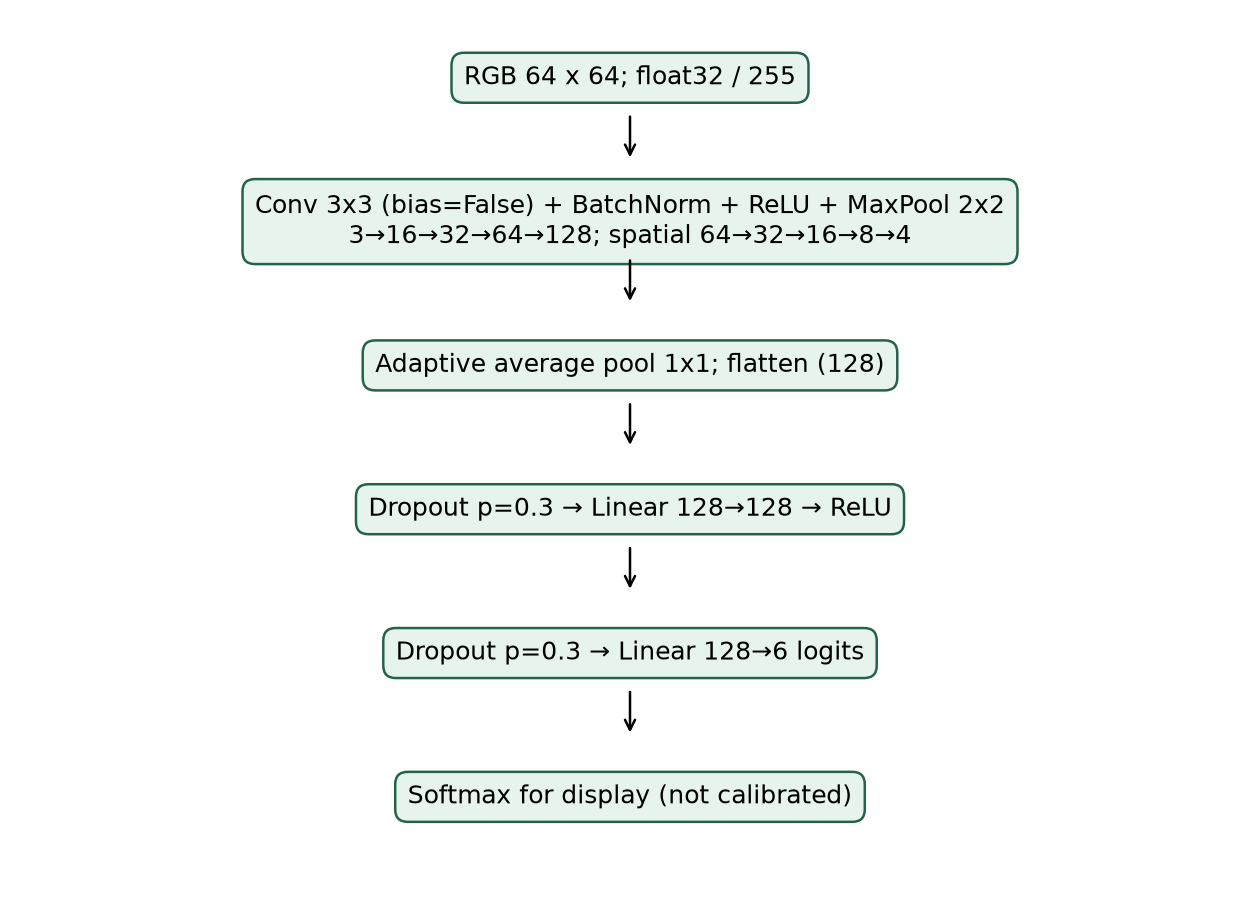
\includegraphics[width=\columnwidth]{architecture.png}
\caption{Actual selected network. The convolution block is repeated four times with the indicated channel progression.}\label{fig:architecture}
\end{figure}
The selected checkpoint is \texttt{models/waste\_cnn.pth}; the implementation is \texttt{starter/student\_core.py}. Safe tensor-only deserialization validates class order, preprocessing metadata, architecture and strict state-dict loading. Its SHA-256 is recorded in \texttt{audit.json}. A real sample executes on CPU with output shape $(1,6)$; CPU and CUDA validation are included in the test package. No architecture replacement or new training was performed.

\section{Experimental Setup}
The original experiments use Adam, base learning rate 0.002, weighted cross-entropy, batch size 32 and 25 epochs with seed 42. ReduceLROnPlateau monitors validation loss. Each run restores the epoch with minimum validation loss; the configuration is selected by validation Macro-F1 among dropout-positive candidates. The selected aug\_none model uses no training augmentation, dropout 0.3 and epoch 24. Baseline geometric augmentation includes flips, rotations up to 28.8 degrees and mild crop/resize; full augmentation also changes brightness and contrast. Deterministic evaluation has no random augmentation. These single-seed ablations cannot establish statistical superiority across training seeds.

\section{Ablation Study}
Table~\ref{tab:ablation} reports validation scores only. Base has four blocks and geometric augmentation. aug\_none removes augmentation; aug\_full adds photometric changes. drop\_0.0 and drop\_0.5 change dropout alone. depth\_2 uses channels (32,64), while depth\_3 uses (16,32,64); these are not simple truncations with identical channel widths. Learning-rate variants use 0.0002 and 0.01. no\_reg disables augmentation and dropout but retains Batch Normalization. Its 0.815 validation Macro-F1 exceeds aug\_none's 0.720, but the architecture rubric explicitly requires dropout greater than zero. This is a constraint-driven trade-off, not evidence that aug\_none is the best unconstrained model. Neither its name nor the existence of dropout proves no\_reg overfits; that claim requires learning-curve and independent generalization evidence. Strong augmentation/dropout may underfit within this fixed training budget.
\begin{table}[t]\centering\caption{Existing validation ablations. D: depth; p: dropout; LR: learning rate.}\label{tab:ablation}
\scriptsize\begin{tabular}{lrrlrr}\hline
Model & D & p & Augmentation & LR & Macro-F1\\\hline
aug\_full & 4 & 0.3 & full & 0.002 & 0.573 \\
aug\_none & 4 & 0.3 & none & 0.002 & 0.720 \\
base & 4 & 0.3 & geometric & 0.002 & 0.641 \\
depth\_2 & 2 & 0.3 & geometric & 0.002 & 0.576 \\
depth\_3 & 3 & 0.3 & geometric & 0.002 & 0.618 \\
drop\_0.0 & 4 & 0.0 & geometric & 0.002 & 0.717 \\
drop\_0.5 & 4 & 0.5 & geometric & 0.002 & 0.583 \\
lr\_1e-2 & 4 & 0.3 & geometric & 0.01 & 0.665 \\
lr\_2e-4 & 4 & 0.3 & geometric & 0.0002 & 0.584 \\
no\_reg & 4 & 0.0 & none & 0.002 & 0.815 \\
\hline\end{tabular}\end{table}

\section{Experimental Results}
The original test benchmark is preserved in Table~\ref{tab:benchmark}. The selected CNN correctly classifies 334/435 images. Its original image-bootstrap 95\% Macro-F1 interval is [0.709,0.799] from 1,000 resamples. This interval quantifies test-image sampling uncertainty, not training-seed variability or domain shift.
\begin{table}[t]\centering\caption{Original held-out test results (435 images).}\label{tab:benchmark}
\begin{tabular}{lrr}\hline Model & Accuracy & Macro-F1\\\hline
Majority class & 0.234 & 0.063\\
Color histogram centroid & 0.384 & 0.353\\
Selected CNN (aug\_none) & 0.768 & 0.757\\\hline\end{tabular}\end{table}
A preliminary 30-image Qwen2.5-VL 3B comparison via Ollama gave CNN 25/30 (83.3\%) and Qwen 20/30 (66.7\%), with original approximate times of 0.01 and 1.28 seconds/image. Small sample size, prompt/output parsing, hardware and timing protocol constrain interpretation. It does not show that CNNs are generally better than vision-language models.

\section{Error Analysis}
Paper and cardboard have the strongest original per-class F1 (0.878 and 0.864). Glass, trash and metal score 0.670, 0.679 and 0.697. Glass-to-metal errors total 16, metal-to-glass 13 and glass-to-plastic 9. Color, silhouettes and reflections can be visually similar; labels and packaging are possible confounds. These observations do not prove causal mechanisms. The 12 highest-confidence wrong predictions score approximately 91\%--99.9\%. A maximum-score threshold of 50\% misses these errors and is not an unknown-object detector. Figure~\ref{fig:cm} shows the newly rerun standard confusion matrix; image galleries and all six scores are saved for inspection. Figure~\ref{fig:errors} shows the most confident errors.
\begin{figure}[t]\centering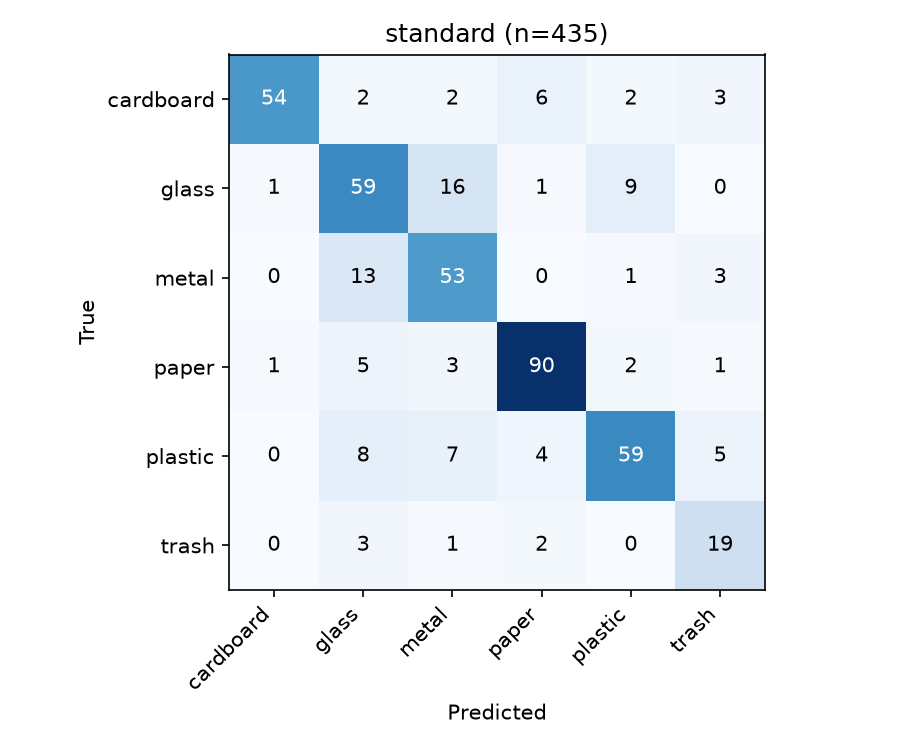
\includegraphics[width=\columnwidth]{../results/stress/standard_confusion.png}\caption{Rerun standard held-out confusion matrix; rows are true classes.}\label{fig:cm}\end{figure}
\begin{figure}[t]\centering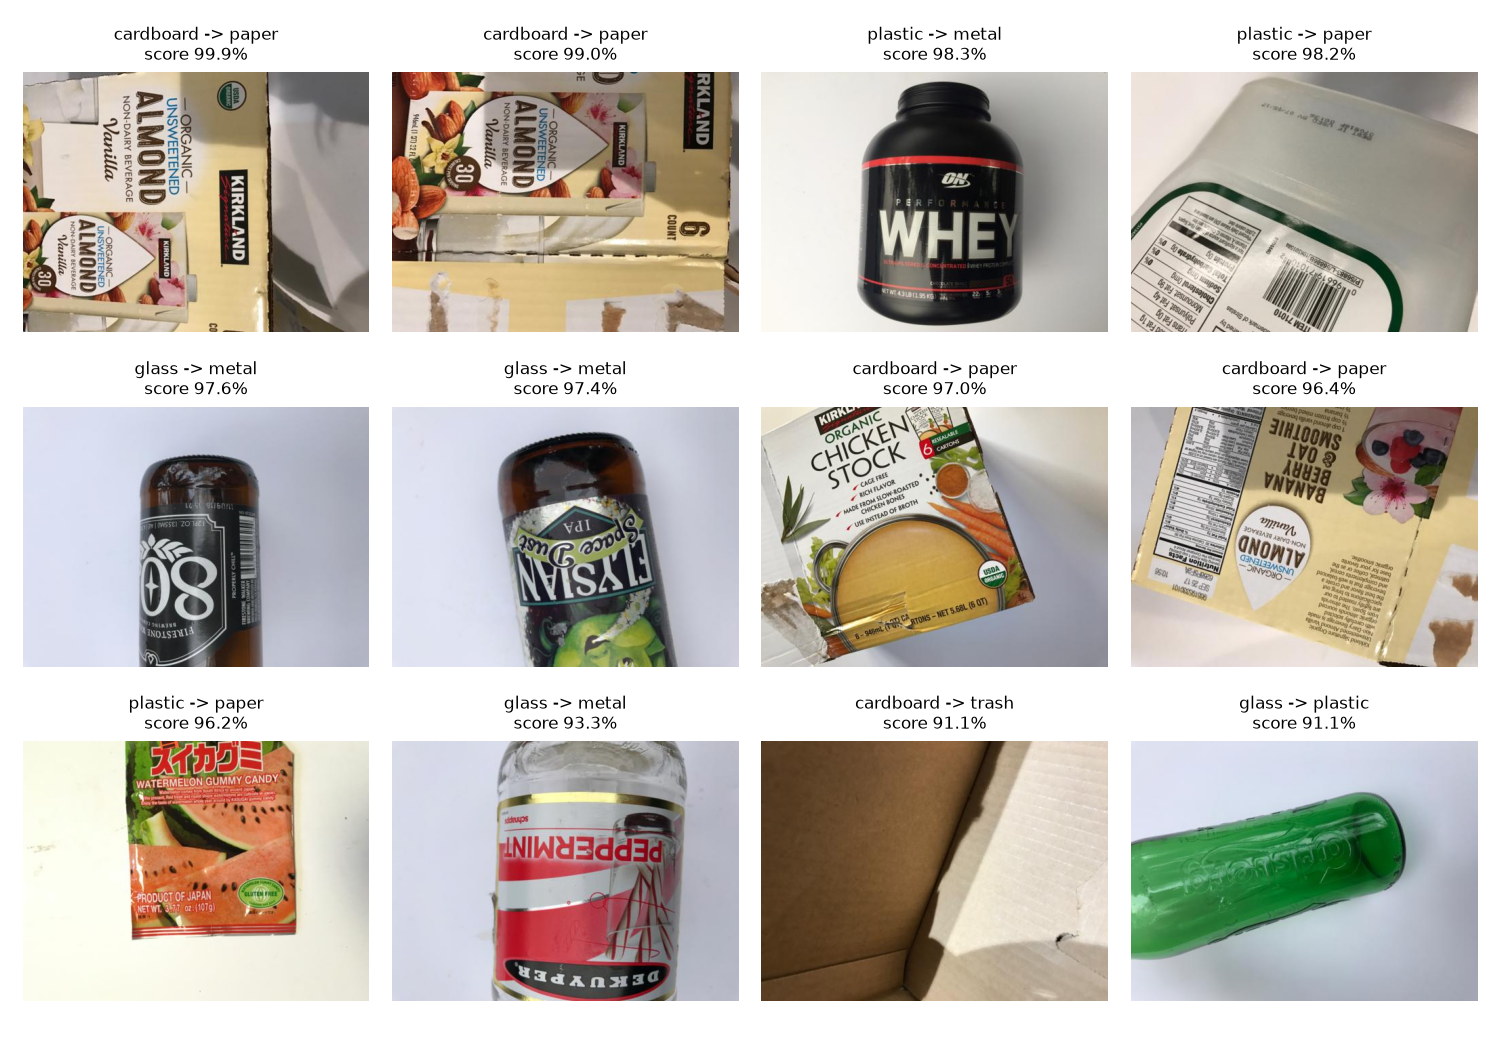
\includegraphics[width=\columnwidth]{../results/stress/standard_high_confidence_errors.png}\caption{Highest-confidence incorrect standard predictions. Scores are not calibrated probabilities.}\label{fig:errors}\end{figure}

\section{AI Product Implementation}
The Streamlit application has four views: Waste Classifier, Model Information, Known Limitations \& Failure Modes, and Robustness Testing. JPEG/PNG uploads undergo byte-size, content-format, integrity and dimension checks before full decoding. Limits are 10 MiB, 20 megapixels and 8192 pixels per side. EXIF orientation is corrected; grayscale converts to RGB; transparency composites on white. These upload-specific adaptations are explicit and are not applied silently to the historical test benchmark. A preview shows format and dimensions before the Predict button executes.
A cached resource loads the selected model once per checkpoint modification. Inference uses evaluation mode and \texttt{torch.inference\_mode()}, CPU or CUDA, and softmax over exactly six finite logits. Six horizontal bars, predicted class and latency appear alongside an educational-use warning. Latency measures batch-one forward plus softmax, excludes decode/resize/transfers and synchronizes CUDA; five warmup passes precede evaluation. It is not end-to-end upload latency.
Educational content lives in a separate JSON file with descriptions, examples, preparation, warnings, local scope and sources. General preparation includes emptying containers and keeping paper dry \cite{epa,ecology}. The Vietnamese Environment Agency describes three source-separation groups: reusable/recyclable, food and other household waste \cite{vietnam}. Six model classes are not six mandated collection bins. Campus location is unconfirmed, and no Hanoi-specific collection acceptance or bin colors are asserted. Users must confirm arrangements with their collector; a prediction never guarantees acceptance or disposal safety.

\section{Stress and Edge Scenario Evaluation}
\subsection{Protocol and Provenance}
The shared evaluator loads the same checkpoint, class order and deterministic preprocessing as the app. A CSV manifest freezes image paths, independent true labels, condition, physical/source identity, capture information, transformation and SHA-256. Each result stores checkpoint/manifest hashes, environment, all six scores, ground truth, prediction and timing. The original files remain unchanged. Macro-F1 always averages the same six classes. Bootstrap intervals are omitted for fewer than 30 source groups or incomplete class coverage. Synthetic variants are clustered by source image for resampling and are not independent new objects. The source-image IDs cannot establish original physical object identity. No challenge data is used to tune the network.
\begin{table}[t]\centering\caption{New evaluations, separate from original benchmark. A: accuracy; F1: Macro-F1.}\label{tab:stress}
\scriptsize\begin{tabular}{lrrr}\hline Condition & n & A & F1\\\hline
standard & 435 & 0.768 & 0.757 \\
complex & 12 & 0.833 & 0.828 \\
low\_light\_blur\_synthetic & 1740 & 0.486 & 0.484 \\
low\_light\_blur\_real & 0 & \multicolumn{2}{c}{Not evaluated} \\
campus\_novel & 0 & \multicolumn{2}{c}{Not evaluated} \\
\hline\end{tabular}\end{table}

\subsection{Standard and Complex Items}
All 435 held-out images are rerun. The new CPU run obtains accuracy 0.7678 and Macro-F1 0.7575; the source-image-bootstrap Macro-F1 interval is [0.7092,0.7994]. Mean forward-plus-softmax latency is 4.11 ms/image. Differences from the original benchmark, if any, are retained rather than edited to match it.
The complex subset contains 12 actual held-out images selected visually before obtaining the new predictions, from the first eight sorted images per class. It includes flattened/printed board, cropped/labeled glass, crumpled foil, printed metal packaging, curled/overlapping printed paper, ridged plastic and wrinkled residual material. It is a descriptive subset overlapping the standard set, not an independent challenge distribution. It does not cover every requested deformation or complex background. Accuracy is 0.8333 and Macro-F1 is 0.8278; with only two examples per class no uncertainty interval or general robustness claim is justified. Errors can be described visually but cannot be attributed causally to a single nuisance factor.

\subsection{Synthetic Low-Light and Blur}
At source resolution, brightness is multiplied by 0.30, contrast by 0.35, defocus uses a Gaussian radius of 2 pixels, and motion uses a horizontal 9-pixel box kernel with edge padding. Each held-out source yields four lossless PNG variants, for 1,740 transformed images. Images are then processed through the unchanged 64-by-64 model transform. Table~\ref{tab:transforms} separates these perturbations. Darkening reduces Macro-F1 to 0.046 and low contrast to 0.192, whereas the two blur settings retain approximately 0.745--0.747. Thus the aggregate score masks substantially different sensitivities. This is a measured response to these chosen perturbation strengths, not a general comparison of camera conditions. These are sensitivity experiments on existing objects, not real phone captures or a substitute for field testing. Figure~\ref{fig:stress} compares the available scenarios and Fig.~\ref{fig:latency} shows their timings.
\begin{table}[t]\centering\caption{Controlled transformations (435 sources each).}\label{tab:transforms}
\begin{tabular}{lrrr}\hline Transform & n & Accuracy & Macro-F1\\\hline
dark & 435 & 0.159 & 0.046 \\
low\_contrast & 435 & 0.276 & 0.192 \\
defocus & 435 & 0.754 & 0.745 \\
motion & 435 & 0.756 & 0.747 \\
\hline\end{tabular}\end{table}
\begin{figure}[t]\centering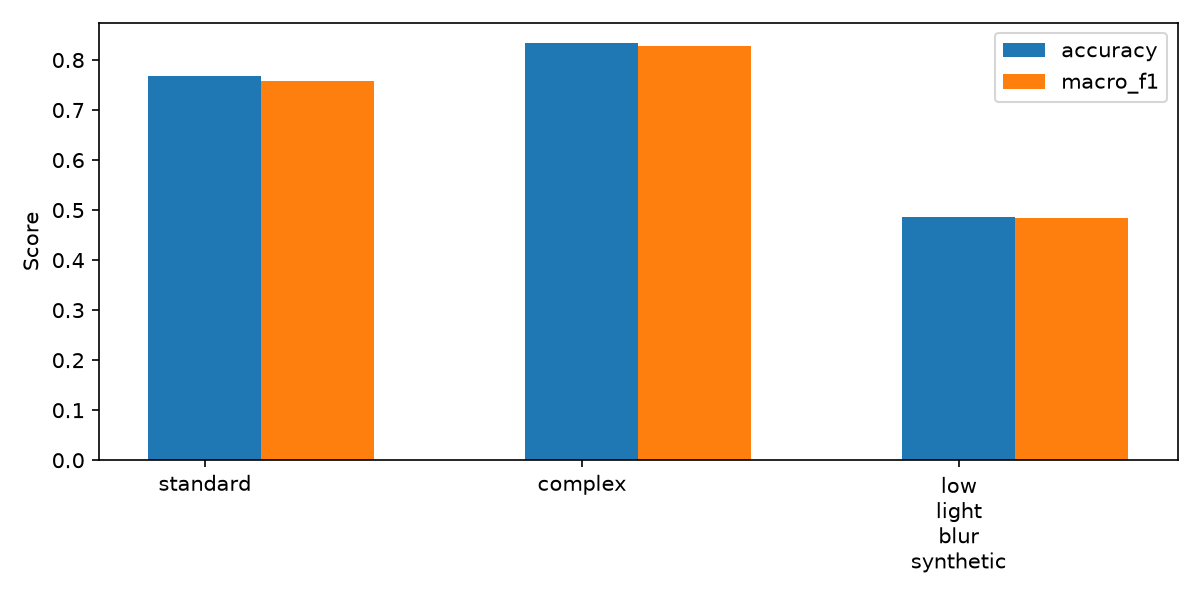
\includegraphics[width=\columnwidth]{../results/stress/scenario_comparison.png}\caption{Available scenario results. The complex subset overlaps standard data; synthetic variants reuse the same source images.}\label{fig:stress}\end{figure}
\begin{figure}[t]\centering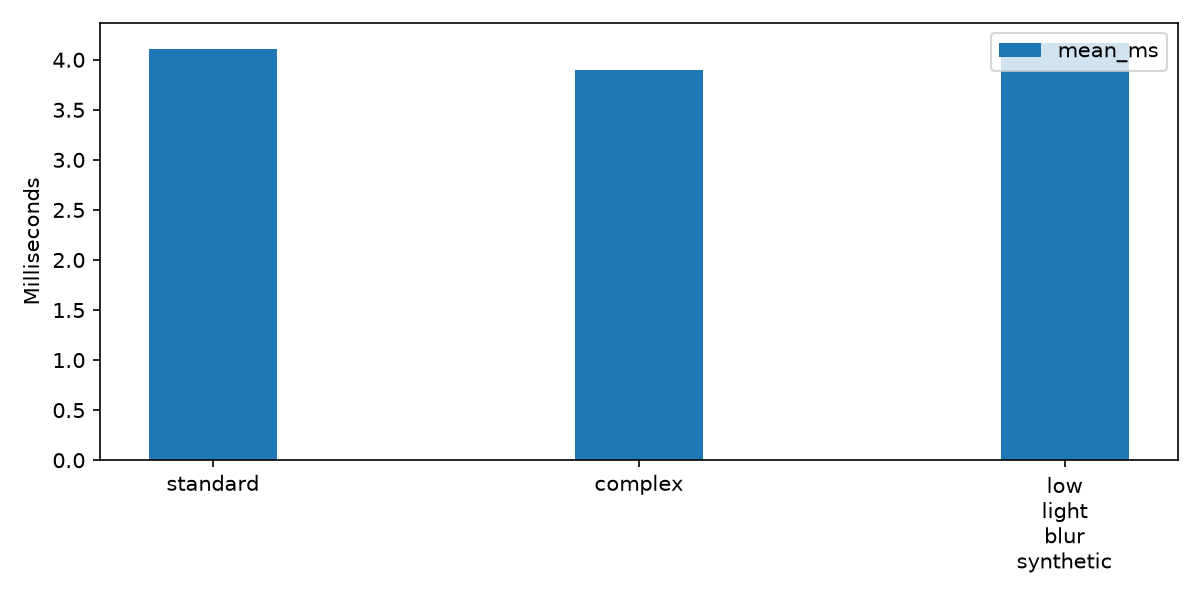
\includegraphics[width=\columnwidth]{../results/stress/latency.png}\caption{New CPU timing with the documented warmed-up batch-one protocol. Hardware-specific measurements are not direct Qwen comparisons.}\label{fig:latency}\end{figure}

\subsection{Real Camera and Novel Campus Conditions}
No genuine camera low-light/blur photographs or novel campus photographs were supplied. These two evaluations remain unexecuted, with zero samples rather than zero performance. Empty manifests, separate directories, a collection checklist and executable evaluator are provided. The team should collect at least five distinct physical items per category when practical, use varied conditions, exclude ambiguous taxonomy cases, independently freeze labels and keep challenge photographs out of training and validation. Avoid identifiable people and private locations. Distinct object IDs prevent duplicate camera/campus evaluation rows. Real camera and synthetic data must remain separate in any updated report. Required crumpled paper, crushed cans, deformed bottles, occlusion and clutter examples still need broader real-photo collection.

\section{Limitations and Future Work}
This is one seed and a limited 25-epoch training budget. Filename-level splits may leak physical objects. Low input resolution removes texture; unknown objects are forced into known labels; softmax is uncalibrated. Convenience subsets and synthetic transformations do not estimate deployment accuracy. Local acceptance depends on the collector and cannot be inferred from appearance alone. Future work should collect an independent campus challenge set, investigate object-grouped splits, add multi-seed evaluation and assess calibration on a separate validation/calibration set. Any threshold or calibration choice must be frozen before the final challenge evaluation. Inference benchmarking should additionally report full upload-to-result latency if needed. These improvements are proposals, not claimed completed experiments.

\section{Conclusion}
The original selected CNN is integrated into a functional, transparent educational product with shared inference and reproducible evaluation. Existing benchmarks and constraint-driven model selection are preserved. Controlled perturbations and a small real-image subset document measurable sensitivity, while genuine campus and real-camera validation remain explicit outstanding inputs. The product supports a defensible demonstration provided these remaining conditions are presented honestly.
\newpage
\bibliographystyle{IEEEtran}
\bibliography{references}
\end{document}
